\chapter{Операции и функции}
\label{sec:development}

Разработанное программное обеспечение предстваляет из себя библиотеку кода,
написанную на языке \csharp{}. Модель проекта не ограничена только данным языком и платформой,
так как в реализации используются только стандартные типы данных и библиотека \rx{}.
\rx{} портированы на множество платформ: \java{}, \javascript{}, \python{} и другие.

В контексте этой главы я хочу рассказать о реализованных в проекте операций реляционной алгебры c некоторыми модификациями,
которые позволяют получить обновляемые проекции. Список реализованных на текущий момент операций:

\begin{itemize}
  \item Select --- проекция;
  \item Where --- выборка;
  \item SelectMany --- проекция элементов в последовательности с последующим объединением;
  \item GroupBy --- группировка элементов по ключу;
  \item Take --- выборка указанного количества первых элементов списка;
  \item Skip --- выборка всех элементов списка кроме указанного количества первых элементов;
  \item Union --- объединение;
  \item Intersect --- пересечение;
  \item Except --- вычитание;
  \item Sort --- сортировка;
  \item Join --- декартово произведение;
  \item Reverse --- отображение в список с обратным порядком;
  \item Distinct --- отображение набора элементов в множество.
\end{itemize}

Также реализовано несколько функций:

\begin{itemize}
  \item Count --- количество элементов;
  \item Max --- максимальный элемент;
  \item Min --- минимальный элемент.
\end{itemize}

\begin{figure}[ht]
\centering
  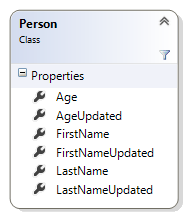
\includegraphics[scale=0.85]{person.png}
  \caption{ Класс Person }
  \label{fig:person}
\end{figure}

Далее я расскажу подробно о каждом реализованном методе из данных списков.
Примеры описанные в листингах помогают понять, как их использовать.
Для упрощения примеров, в каждом будет использоваться набор элементов Person(см. рисунок~\ref{fig:person}), который содержит свойства FirstName(Имя), LastName(Фамилия), Age(Возраст).
Также класс содержит генераторы событий, которые позволяют узнать, когда и какое свойство изменилось.

\section{Select}
\label{sub:development:select}

Select --- проецирует элемент последовательности в новыю форму.
В данном случае метод принимает два параметра: selector --- функция преобразования,
применяемая к каждому элементу, updaterSelector --- функция преобразования,
применяемая к каждому элементу, которая получает генератор событий изменения элемента.

\begin{lstlisting}[style=csharpinlinestyle, caption={Пример использования Select}, label=lst:practice:development:select]
  IObservableCollection<Person> collection = new ObservableCollection<Person>(); // create collection
  IObservableReadOnlyCollection<string> names = collection.SelectRc(x => x.FirstName, x => x.FirstNameChanged.Select(_ => x)); // create projection
  IDisposable sub = names.CollectionChanged.Subscribe(
    x => x.Match(
      onInsert: y => { Console.WriteLine(y.Item); },
      onRemove: y => { },
      onReplace: y => { Console.WriteLine($"{y.OldItem} -> {y.NewItem}"); },
      onReset: y => { },
      onEmpty: y => { })); \\ create subscription

  collection.Add(new Person() { FirstName = "Alan", LastName = "Wake", Age = 32 }); // output: Alan
  Person vader = new Person() { FirstName = "Darth", LastName = "Vader", Age = 45 };
  collection.Add(vader); // output: Darth

  vader.FirstName = "Anakin"; // output: Darth -> Anakin
\end{lstlisting}

В листинге~\ref{lst:practice:development:select} создается наблюдаемая коллекция. Затем создается проекция и обработчик событий,
который обрабатывает событие добавления элементов в коллекцию и замену элементов.
Проекция выбирает имена людей. При изменении имени у объекта Person изменится и проекция.
Как можно заметить операция реагирует на изменение проекции, если передать ей соответствующий генератор событий.

\section{Where}
\label{sub:development:where}

Where --- выполняет фильтрацию последовательности значений на основе заданного предиката.
В данном случае метод принимает два параметра: predicate --- функция для проверки каждого элемента на соответствие условию,
применяемая к каждому элементу, updaterSelector --- функция преобразования,
применяемая к каждому элементу, которая получает генератор событий изменения элемента.

\begin{lstlisting}[style=csharpinlinestyle, caption={Пример использования Where}, label=lst:practice:development:where]
  IObservableCollection<Person> collection = new ObservableCollection<Person>(); // create collection
  IObservableReadOnlyCollection<Person> olderThan40 = collection.WhereRc(x => x.Age > 40, x => x.AgeChanged.Select(_ => x)); // create filter
  IDisposable sub = olderThan40.CollectionChanged.Subscribe(
    x => x.Match(
      onInsert: y => { Console.WriteLine($"added {y.Item.FirstName}"); },
      onRemove: y => { Console.WriteLine($"removed {y.Item.FirstName}"); },
      onReplace: y => { },
      onReset: y => { },
      onEmpty: y => { })); \\ create subscription

  Person wake = new Person() { FirstName = "Alan", LastName = "Wake", Age = 32 };
  collection.Add(wake);
  Person vader = new Person() { FirstName = "Darth", LastName = "Vader", Age = 45 };
  collection.Add(vader); // output: added Darth

  wake.Age = 45; // output: added Alan
  vader.Age = 6; // output: removed Darth
\end{lstlisting}

В листинге~\ref{lst:practice:development:where} создается наблюдаемая коллекция. Затем создается выборка, зависящая от возраста. Затем создается обработчик событий,
который обрабатывает событие добавления и удаления элементов. Полученный фильтр обрабатывает добавленные в исходную коллекцию элементы и реагирует на изменение критерия для предиката.
Как можно заметить операция реагирует на изменение исходной коллекции и содержимого элементов, если передать ей соответствующий генератор событий для предиката.

\section{SelectMany}
\label{sub:development:select_many}

SelectMany --- проецирует каждый элемент последовательности в IObservableReadOnlyCollection<T> и объединяет результирующие последовательности в одну последовательность.
В данном случае метод принимает один параметр: selector --- функция преобразования, применяемая к каждому элементу.

\begin{lstlisting}[style=csharpinlinestyle, caption={Пример использования SelectMany}, label=lst:practice:development:select_many]
  IObservableCollection<Person> collection = new ObservableCollection<Person>(); // create collection
  IObservableReadOnlyCollection<Person> persons = collection.SelectManyRc(x => collection); // create projection
  IDisposable sub = persons.CollectionChanged.Subscribe(
    x => x.Match(
      onInsert: y => { Console.WriteLine($"added {y.Item.FirstName}"); },
      onRemove: y => { Console.WriteLine($"removed {y.Item.FirstName}"); },
      onReplace: y => { },
      onReset: y => { },
      onEmpty: y => { })); \\ create subscription

  Person wake = new Person() { FirstName = "Alan", LastName = "Wake", Age = 32 };
  collection.Add(wake); // output: added Alan

  Person vader = new Person() { FirstName = "Darth", LastName = "Vader", Age = 45 };
  collection.Add(vader); // output: added Darth
                         // output: added Alan
                         // output: added Darth
\end{lstlisting}

В листинге~\ref{lst:practice:development:select_many} создается наблюдаемая коллекция. Затем создается проекция, которая отобржает каждый элемент в исходную коллекцию.
Затем создается обработчик событий, который обрабатывает событие добавления и удаления элементов.
Полученная проекция обрабатывает события исходной коллекции и на изменения коллекций полученных из функции преобразования.
Т. е. если удалить элемент из исходной коллекции, то удалятся все элементы, которые соответсвовали проекции этого элемента.
Если удалить элемент из проекции элемента, то из результирущей наблюдаемой коллекции удалится этот же самый элемент.

\section{GroupBy}
\label{sub:development:group_by}

GroupBy --- cоздает наблюдаемую коллекцию ключей, каждый из которых сопоставлен с одним или несколькими значениями в соответствии с заданной функцией выбора ключа.
Метод принимает два параметр: keySelector --- функция, извлекающая ключ из каждого элемента, updaterSelector --- функция преобразования,
применяемая к каждому элементу, которая получает генератор событий изменения ключа элемента.

\begin{lstlisting}[style=csharpinlinestyle, caption={Пример использования GroupBy}, label=lst:practice:development:group_by]
  IObservableCollection<Person> collection = new ObservableCollection<Person>(); // create collection
  IObservableLookup<char, Person> persons = collection.GroupBy(x => x.LastName[0], x => x.LastNameChanged.Select(_ => x)); // create observable lookup
  IDisposable sub = persons.CollectionChanged.Subscribe(
    x => x.Match(
      onInsert: y => { Console.WriteLine($"added {y.Item.Key}"); },
      onRemove: y => { Console.WriteLine($"removed {y.Item.Key}"); },
      onReplace: y => { },
      onReset: y => { },
      onEmpty: y => { })); \\ create subscription

  Person wake = new Person() { FirstName = "Alan", LastName = "Wake", Age = 32 };
  collection.Add(wake); // output: added W

  Person vader = new Person() { FirstName = "Darth", LastName = "Vader", Age = 45 };
  collection.Add(vader); // output: added V

\end{lstlisting}

В листинге~\ref{lst:practice:development:group_by} создается наблюдаемая коллекция. Затем создается словарь, где каждому элементу соответвует наблюдаемая коллекция эллементов.
Затем создается обработчик событий, который обрабатывает событие добавления и удаления элементов.
Полученный словарь реагирует на добавление новых ключей и элементов в коллекции для каждого ключа. Если для ключа отсутствуют элементы, которые ему соответсвуют --- он удаляется из словаря.

\section{Take и Skip}
\label{sub:development:take_skip}

Take и Skip --- cоздают наблюдаемый список, который соответсвует подсписку исходного. В данной реализации эти опрерации объединены в одну SkipAndTake.
Метод принимает два параметр: skip --- количество элементов от начала списка требуется пропустить, take --- максимальное количество элементов после пропущенных, которое можно взять.

\begin{lstlisting}[style=csharpinlinestyle, caption={Пример использования SkipAndTake}, label=lst:practice:development:skip_and_take]
  IObservableList<Person> list = new ObservableList<Person>(); // create list
  ObservableValue<int> skip = new ObservableValue<int>(0);
  ObservableValue<int> take = new ObservableValue<int>(1);
  IObservableReadOnlyList<Person> persons = list.SkipAndTakeRl(skip, take); // create sublist
  IDisposable sub = persons.ListChanged.Subscribe(
    x => x.Match(
      onInsert: y => { Console.WriteLine($"added {y.Item.FirstName}"); },
      onRemove: y => { Console.WriteLine($"removed {y.Item.FirstName}"); },
      onReplace: y => { },
      onMove: y => { }
      onReset: y => { },
      onEmpty: y => { })); \\ create subscription

  Person wake = new Person() { FirstName = "Alan", LastName = "Wake", Age = 32 };
  collection.Add(wake); // output: added Alan

  Person vader = new Person() { FirstName = "Darth", LastName = "Vader", Age = 45 };
  collection.Add(vader);

  skip.Value = 1; // output: removed Alan
                  // output: added Darth
\end{lstlisting}

В листинге~\ref{lst:practice:development:skip_and_take} создается наблюдаемая коллекция. Затем создаются объекты, у которых можно менять значение и подписаться на его изменение.
Затем создается подсписок, у которого пропускается 0 элементов и берется максимум 1. При добавлении первой записи, она также попадает в подсписок.
При добавлении второй, места в подсписке нет, так как он ограничен одним элементом. Далее мы изменяем количество элементов, которое мы хотим пропускать с 0 до 1. Это значит что запись Alan удалится
из подсписка, а Darth добавится. Обработка событий обновления исходного списка идет с сохранением позиций элементов относительно друг друга.

\section{Union}
\label{sub:development:union}

Union --- находит объединения наборов двух последовательностей, используя компаратор проверки на равенство.
Метод принимает три параметра: second --- вторую последовательность элементов такого же типа, что и исходная,
comparer --- функция для сравнения элементов, updaterSelector --- функция преобразования, применяемая к каждому элементу, которая получает генератор событий изменения элемента.

\begin{lstlisting}[style=csharpinlinestyle, caption={Пример использования Union}, label=lst:practice:development:union]
  IObservableCollection<Person> collection1 = new ObservableCollection<Person>(); // create collection1
  IObservableCollection<Person> collection2 = new ObservableCollection<Person>(); // create collection2
  IObservableReadOnlyCollection<Person> persons = collection1.UnionRc(collection2, EqualityComparer<Person>.Default, x => Observable.Never<Person>()); // create union
  IDisposable sub = persons.CollecionChanged.Subscribe(
    x => x.Match(
      onInsert: y => { Console.WriteLine($"added {y.Item.FirstName}"); },
      onRemove: y => { Console.WriteLine($"removed {y.Item.FirstName}"); },
      onReplace: y => { },
      onMove: y => { }
      onReset: y => { },
      onEmpty: y => { })); \\ create subscription

  Person wake = new Person() { FirstName = "Alan", LastName = "Wake", Age = 32 };
  collection1.Add(wake); // output: added Alan

  Person vader = new Person() { FirstName = "Darth", LastName = "Vader", Age = 45 };
  collection2.Add(vader); // output: added Darth
\end{lstlisting}

В листинге~\ref{lst:practice:development:union} создается две наблюдаемые коллекции для объектов Person. Затем создается наблюдаемая коллекция, которая является объединением исходных двух.
При добавлении элементов в какую-либо из исходных коллекций, элементы добавляются в результирующую. Таким образом можно объединять несколько коллекций и создавать глобальные коллекции,
которые следят, например, за списком контактов из разных учетных записей пользователя.

\section{Intersect}
\label{sub:development:intersect}

Intersect --- находит пересечение наборов двух последовательностей, используя компаратор проверки на равенство.
Метод принимает три параметра: second --- вторую последовательность элементов такого же типа, что и исходная,
comparer --- функция для сравнения элементов, updaterSelector --- функция преобразования, применяемая к каждому элементу, которая получает генератор событий изменения элемента.

\begin{lstlisting}[style=csharpinlinestyle, caption={Пример использования Intersect}, label=lst:practice:development:intersect]
  IObservableCollection<Person> collection1 = new ObservableCollection<Person>(); // create collection1
  IObservableCollection<Person> collection2 = new ObservableCollection<Person>(); // create collection2
  IObservableReadOnlyCollection<Person> persons = collection1.IntersectRc(collection2, EqualityComparer<Person>.Default, x => Observable.Never<Person>()); // create intersect
  IDisposable sub = persons.CollecionChanged.Subscribe(
    x => x.Match(
      onInsert: y => { Console.WriteLine($"added {y.Item.FirstName}"); },
      onRemove: y => { Console.WriteLine($"removed {y.Item.FirstName}"); },
      onReplace: y => { },
      onMove: y => { }
      onReset: y => { },
      onEmpty: y => { })); \\ create subscription

  Person wake = new Person() { FirstName = "Alan", LastName = "Wake", Age = 32 };
  Person vader = new Person() { FirstName = "Darth", LastName = "Vader", Age = 45 };
  Person geralt = new Person() { FirstName = "Geralt", LastName = "From Rivia", Age = 60 };

  collection1.Add(wake);
  collection1.Add(vader);
  collection2.Add(vader); // output: added FirstName
  collection2.Add(geralt)
\end{lstlisting}

В листинге~\ref{lst:practice:development:intersect} создается две наблюдаемые коллекции для объектов Person. Затем создается наблюдаемая коллекция, которая является пересечением исходных двух.
При добавлении элементов в какую-либо из исходных коллекций, алгоритм операции используюет компаратор определяет вхождение элемента и решает добавлять или не добавлять в результирующую коллекцию.
Результат операции сходен с результатом выполнения Intersect из LINQ. Таким образом можно находить пересечения нескольких коллекций.

\section{Except}
\label{sub:development:except}

Except --- находит разницу наборов двух последовательностей, используя компаратор проверки на равенство.
Метод принимает три параметра: second --- вторую последовательность элементов такого же типа, что и исходная,
comparer --- функция для сравнения элементов, updaterSelector --- функция преобразования, применяемая к каждому элементу, которая получает генератор событий изменения элемента.

\begin{lstlisting}[style=csharpinlinestyle, caption={Пример использования Except}, label=lst:practice:development:except]
  IObservableCollection<Person> collection1 = new ObservableCollection<Person>(); // create collection1
  IObservableCollection<Person> collection2 = new ObservableCollection<Person>(); // create collection2
  IObservableReadOnlyCollection<Person> persons = collection1.ExceptRc(collection2, EqualityComparer<Person>.Default, x => Observable.Never<Person>()); // create Except
  IDisposable sub = persons.CollecionChanged.Subscribe(
    x => x.Match(
      onInsert: y => { Console.WriteLine($"added {y.Item.FirstName}"); },
      onRemove: y => { Console.WriteLine($"removed {y.Item.FirstName}"); },
      onReplace: y => { },
      onMove: y => { }
      onReset: y => { },
      onEmpty: y => { })); \\ create subscription

  Person wake = new Person() { FirstName = "Alan", LastName = "Wake", Age = 32 };
  Person vader = new Person() { FirstName = "Darth", LastName = "Vader", Age = 45 };
  Person geralt = new Person() { FirstName = "Geralt", LastName = "From Rivia", Age = 60 };

  collection1.Add(wake); // output: added Alan
  collection1.Add(vader); // output: added Darth
  collection2.Add(vader); // output: removed Darth
  collection2.Add(geralt)
\end{lstlisting}

В листинге~\ref{lst:practice:development:except} создается две наблюдаемые коллекции для объектов Person. Затем создается наблюдаемая коллекция, которая является разницей множеств исходных двух.
При добавлении элементов в какую-либо из исходных коллекций, алгоритм операции используюет компаратор определяет вхождение элемента и решает добавлять или не добавлять в результирующую коллекцию.
Сначала добавляется Alan в первую коллекцию --- разница первой и второй теперь Alan. Затем добавляется Darth --- разница становится Alan и Darth.
При добавлении Darth во вторую коллекцию, он удалится из результирующей, так как он был в первой и согласно правилам вычитания множеств: должен отсутствовать в результате.
Результат операции сходен с результатом выполнения Except из LINQ.

\section{Sort}
\label{sub:development:sort}

Sort --- создает сортированный список согласно критерию и компаратору.
Метод принимает три параметра: selector --- функция, которая строит отображения критерия для сравнения, comparer --- компаратор для критериев,
updaterSelector --- функция преобразования, применяемая к каждому элементу, которая получает генератор событий изменения элемента.

\begin{lstlisting}[style=csharpinlinestyle, caption={Пример использования Sort}, label=lst:practice:development:sort]
  IObservableCollection<Person> collection = new ObservableCollection<Person>(); // create collection
  IObservableReadOnlyList<Person> persons = collection.SortRc(x => x.Age, Comparer<uint>.Default, x => x.AgeUpdated.Select(_ => x)); // create sort
  IDisposable sub = persons.ListChanged.Subscribe(
    x => x.Match(
      onInsert: y => { Console.WriteLine($"added {y.Item.FirstName} to {y.Index}"); },
      onRemove: y => { Console.WriteLine($"removed {y.Item.FirstName} from {y.Index}"); },
      onReplace: y => { },
      onMove: y => { }
      onReset: y => { },
      onEmpty: y => { })); \\ create subscription

  Person vader = new Person() { FirstName = "Darth", LastName = "Vader", Age = 45 };
  Person wake = new Person() { FirstName = "Alan", LastName = "Wake", Age = 32 };
  Person geralt = new Person() { FirstName = "Geralt", LastName = "From Rivia", Age = 60 };

  collection.Add(vader); // output: added Darth to 0
  collection.Add(wake); // output: added Alan to 0
  collection.Add(geralt); // output: added Geralt to 2
  // result [Alan(32), Darth(45), Geralt(60)]
\end{lstlisting}

В листинге~\ref{lst:practice:development:sort} создается коллекция для объектов Person. Затем создается список, в котором записи сортируются согласно возрасту в порядке возрастания.
При добавлении элементов в исходный список, операция определяет позицию для нового элемента согласно компаратору.
Сначала добавляется Darth в первую коллекцию --- его позиция будет 0. Затем добавляется Alan --- его возраст мешьне чем Darth и поэтому его позиция будет 0, а Darth сдвинется на позицию 1.
И наконец Geralt вставится в последнюю позицию. В результате возрасты персонажей будут 32, 45 и 60 соответсвенно.

\section{Join}
\label{sub:development:join}

Join --- Устанавливает корреляцию между элементами двух последовательностей на основе сопоставления ключей.
Метод принимает семь параметров:

\begin{itemize}
  \item inner --- последовательность, соединяемая с исходной последовательностью;
  \item outerKeySelector --- функция, извлекающая ключ соединения из каждого элемента первой последовательности;
  \item outerKeyUpdated --- функция, извлекающая генератой событий изменения ключа для первой коллекции;
  \item innerKeySelector --- функция, извлекающая ключ соединения из каждого элемента второй последовательности;
  \item innerKeyUpdated --- функция, извлекающая генератой событий изменения ключа для второй коллекции;
  \item resultSelector --- функция для создания результирующего элемента для пары соответствующих элементов;
  \item comparer --- функция для хэширования и сравнения ключей.
\end{itemize}

\begin{lstlisting}[style=csharpinlinestyle, caption={Пример использования Join}, label=lst:practice:development:join]
  IObservableCollection<Person> collection1 = new ObservableCollection<Person>(); // create collection1
  IObservableCollection<Person> collection2 = new ObservableCollection<Person>(); // create collection2
  IObservableReadOnlyCollection<string> persons = collection1.JoinRc(
    collection2,
    x => x.Age,
    x => Observable.Never<Person>(),
    x => x.Age,
    x => Observable.Never<Person>(),
    (x, y) => $"{x.FirstName} + {y.FirstName}",
    EqualityComparer<uint>.Default); // create join

  IDisposable sub = persons.CollecionChanged.Subscribe(
    x => x.Match(
      onInsert: y => { Console.WriteLine($"added {y.Item}"); },
      onRemove: y => { Console.WriteLine($"removed {y.Item}"); },
      onReplace: y => { },
      onMove: y => { }
      onReset: y => { },
      onEmpty: y => { })); \\ create subscription

  Person wake = new Person() { FirstName = "Alan", LastName = "Wake", Age = 32 };
  Person vader = new Person() { FirstName = "Darth", LastName = "Vader", Age = 45 };
  Person geralt = new Person() { FirstName = "Geralt", LastName = "From Rivia", Age = 45 };

  collection1.Add(wake);
  collection1.Add(vader);
  collection2.Add(vader); // output: added Darth + Darth
  collection2.Add(geralt) // output: added Darth + Geralt
\end{lstlisting}

В листинге~\ref{lst:practice:development:join} создается две наблюдаемые коллекции для объектов Person. Затем создается наблюдаемая коллекция,
которая является декартовывым произведением с фильтром(inner join) исходных двух. В данном случае ключом является возраст персонажей.
При добавлении элементов в какую-либо из исходных коллекций, алгоритм извлекает ключ и сравнивает его с уже существующмими ключами. Если нужно создается новый элемент и строится проекция
Результат операции сходен с результатом выполнения Join из LINQ.

\section{Reverse}
\label{sub:development:reverse}

Reverse --- создает список согласно c порядком элементов обратным исходному.
Метод не принимает параметров.

\begin{lstlisting}[style=csharpinlinestyle, caption={Пример использования Reverse}, label=lst:practice:development:reverse]
  IObservableList<Person> list = new ObservableLit<Person>(); // create list
  IObservableReadOnlyList<Person> persons = list.ReverseRl(); // create reversed list
  IDisposable sub = persons.ListChanged.Subscribe(
    x => x.Match(
      onInsert: y => { Console.WriteLine($"added {y.Item.FirstName} to {y.Index}"); },
      onRemove: y => { Console.WriteLine($"removed {y.Item.FirstName} from {y.Index}"); },
      onReplace: y => { },
      onMove: y => { }
      onReset: y => { },
      onEmpty: y => { })); \\ create subscription

  Person vader = new Person() { FirstName = "Darth", LastName = "Vader", Age = 45 };
  Person wake = new Person() { FirstName = "Alan", LastName = "Wake", Age = 32 };
  Person geralt = new Person() { FirstName = "Geralt", LastName = "From Rivia", Age = 60 };

  list.Add(vader); // output: added Darth to 0
  list.Add(wake); // output: added Alan to 0
  list.Add(geralt); // output: added Geralt to 0
  // result [Geralt, Alan, Darth]
\end{lstlisting}

В листинге~\ref{lst:practice:development:reverse} создается список для объектов Person. Затем создается список, в котором записи сортируются в обратном порядке.
При добавлении элементов в исходный список, элементы в результирующем получают отраженный индекс. Например, добавление в конец списка вызывает добавление в начало результирующего списка.
Результать операции сходен с результатом выполнения Reverse из LINQ, с тем лишь ограничением, что применяется только для списков.

\section{Distinct}
\label{sub:development:distinct}

Distinct --- возвращает различающиеся элементы последовательности, используя указанный компаратор для сравнения значений.
Метод принимает два параметра: comparer --- функция для сравнения элементов, updaterSelector --- функция преобразования, применяемая к каждому элементу, которая получает генератор событий изменения элемента.

\begin{lstlisting}[style=csharpinlinestyle, caption={Пример использования Distinct}, label=lst:practice:development:distinct]
  IObservableCollection<Person> collection = new ObservableCollection<Person>(); // create collection
  IObservableReadOnlyCollection<Person> persons = collection.DistinctRc(collection, EqualityComparer<Person>.Default, x => Observable.Never<Person>()); // create distinct
  IDisposable sub = persons.CollecionChanged.Subscribe(
    x => x.Match(
      onInsert: y => { Console.WriteLine($"added {y.Item.FirstName}"); },
      onRemove: y => { Console.WriteLine($"removed {y.Item.FirstName}"); },
      onReplace: y => { },
      onMove: y => { }
      onReset: y => { },
      onEmpty: y => { })); \\ create subscription

  Person wake = new Person() { FirstName = "Alan", LastName = "Wake", Age = 32 };
  Person vader = new Person() { FirstName = "Darth", LastName = "Vader", Age = 45 };

  collection.Add(wake); // output: added Alan
  collection.Add(vader); // output: added Darth
  collection.Add(vader); // output: added Darth
  collection.Remove(wake) // output: removed Alan

\end{lstlisting}

В листинге~\ref{lst:practice:development:distinct} создается наблюдаемая коллекция для объектов Person. Затем создается наблюдаемая коллекция, которая является набором уникальных элементов из исходной.
При добавлении элементов равных относительно компаратора, в результирующую коллекцию добавится лишь один и будет существовать, пока в исходной коллекции будет находится хотя бы одна его копия.

\section{Count}
\label{sub:development:count}

Count --- функция, которая возвращает число равное количеству элементов коллекции, обновляемое с изменением коллекции.
Метод не принимает параметров.

\begin{lstlisting}[style=csharpinlinestyle, caption={Пример использования Count}, label=lst:practice:development:count]
  IObservableCollection<Person> collection = new ObservableCollection<Person>(); // create collection
  ObservableValue<int> count = collection.CountRc(); // create count
  IDisposable sub = count.ValueChanged.Subscribe(
    x => { Console.WriteLine($"count = {x}"); }); // create subscription

  Person vader = new Person() { FirstName = "Darth", LastName = "Vader", Age = 45 };
  Person wake = new Person() { FirstName = "Alan", LastName = "Wake", Age = 32 };
  Person geralt = new Person() { FirstName = "Geralt", LastName = "From Rivia", Age = 60 };

  collection.Add(vader); // output: count = 1
  collection.Add(wake); // output: count = 2
  collection.Add(geralt); // output: count = 3
\end{lstlisting}

В листинге~\ref{lst:practice:development:sort} создается коллекция для объектов Person. Затем вычисляется функция Count, значение которой изменяется вместе с изменением исходной коллекции.

\section{Min и Max}
\label{sub:development:min_max}

Min и Max --- функции вычисляющие минимум и максимум соответсвенно.
Метод принимает три параметра: selector --- функция, которая строит отображения критерия для сравнения, comparer --- компаратор для критериев,
updaterSelector --- функция преобразования, применяемая к каждому элементу, которая получает генератор событий изменения элемента.

\begin{lstlisting}[style=csharpinlinestyle, caption={Пример использования Min и Max}, label=lst:practice:development:min_max]
  IObservableCollection<Person> collection = new ObservableCollection<Person>(); // create collection
  ObservableValue<Person?> max = collection.MaxRc(x => x.Age, Comparer<uint>.Default, x => x.AgeUpdated.Select(_ => x)); // create max
  ObservableValue<Person?> min = collection.MinRc(x => x.Age, Comparer<uint>.Default, x => x.AgeUpdated.Select(_ => x)); // create min

  IDisposable sub1 = max.ValueChanged.Subscribe(
    x => { Console.WriteLine($"max age = {x?.Age}"); }); // create subscription
  IDisposable sub2 = min.ValueChanged.Subscribe(
    x => { Console.WriteLine($"min age = {x?.Age}"); }); // create subscription

  Person vader = new Person() { FirstName = "Darth", LastName = "Vader", Age = 45 };
  Person wake = new Person() { FirstName = "Alan", LastName = "Wake", Age = 32 };
  Person geralt = new Person() { FirstName = "Geralt", LastName = "From Rivia", Age = 60 };

  collection.Add(vader); // output: max age = 45
                         // output: min age = 45
  collection.Add(wake); // output: min age = 32
  collection.Add(geralt); // output: max age = 60
\end{lstlisting}

В листинге~\ref{lst:practice:development:min_max} создается коллекция для объектов Person. Затем вычисляются функции Max и Min.
Результат функции пересчитывается при изменении исходной коллекции или её элементов согласно компаратору. Если коллекция пуста, то значение функций примет null.
